\chapter{Introduction}

Computers, in various forms, have become an integral aspect of human daily life. Their ability to tackle a diverse range of tasks, coupled with their efficiency, has significantly expanded their applicability across various fields in recent years. Notably, in the field of medicine, computers have played and continue to play a crucial role, leveraging their potential to assist medical experts in the analysis and annotation of medical data. The capacity to comprehend both textual and visual information is a pivotal feature central to models that can assist medical experts in their daily tasks.

The interaction with medical images by means of written questions holds particular importance, as it facilitates an evaluation of the machine's actual understanding of the information and its ability to reason effectively to provide accurate answers. Within this introductory chapter, we delve into the breakthroughs and concepts that have paved the way for the extensive capabilities computers offer broadly in diverse scenarios and specifically in the medical domain. This exploration is done drawing from the essence of Alan Turing's groundbreaking work about intelligent machines. 

\newpage


\section{Reading Words, Seeing Worlds and Asking Questions}
\label{sec:reading_words_seeing_worlds}

\subsection{Thinking Machines}

% Early computing devices and analog computers
The history of devices capable of aiding in computational tasks extends back at least four millennia, beginning with the creation of the abacus~\cite{flegg1989numbers}. Evolving from this rudimentary counting tool, subsequent centuries revealed more intricate ancient mechanical devices, such as the Antikythera mechanism~\cite{edmunds2014antikythera} and the astrolabe~\cite{north1974astrolabe}, originating from ancient Greece and utilized for astronomical purposes. In more recent history, the seventeenth-century introduction of the slide rule represented a significant step toward more efficient mathematical operations~\cite{stoll2006slide}. While these devices proved useful, their design centered around task-specific manipulation, where the instructions they executed were pre-defined either within the device or by the operator at the time of execution.

% On first computers
Charles Babbage, acknowledged as the father of the computer, introduced a more flexible computing system in the early nineteenth century. His mechanical computer was \textit{programmable}, allowing for the sequential execution of an ordered collection of instructions (\textit{i.e., a program}) defined by the user for a specific task. The program, along with any input data, was provided to the device using punched cards~\cite{kim1999ada}. This concept of programmable computers persisted, but the implementation transitioned from mechanical operation to vacuum tubes and subsequently to transistors. At the time, the first electronic computers were large and heavy devices that only some institutions had the privilege to utilize. 

% Start with Turing 1950 paper, i.e. machines pretending to be humans
In 1950, Alan Turing published a work titled Computing Machinery and Intelligence~\cite{turing2009computing}, where he addressed the question ``Can machines think?" by framing it as the outcome of a game. The game, known as the imitation game or the Turing test, involves three participants in isolation, as illustrated in Fig.~\ref{fig:imitation_game}: a machine (A), a person (B) and another person assuming the role of interrogator (C). In this scenario, the interrogator uses text-based communication to interact with A and B through questions and answers. The goal for A is to behave in a manner indistinguishable from a human during the conversation. Following the game, interrogator C indicates which participant corresponds to the computer and which is human. From this perspective, if C incorrectly classifies the participants with high probability, the machine is considered intelligent or capable of thinking.

\begin{figure}[!ht]
\begin{center}
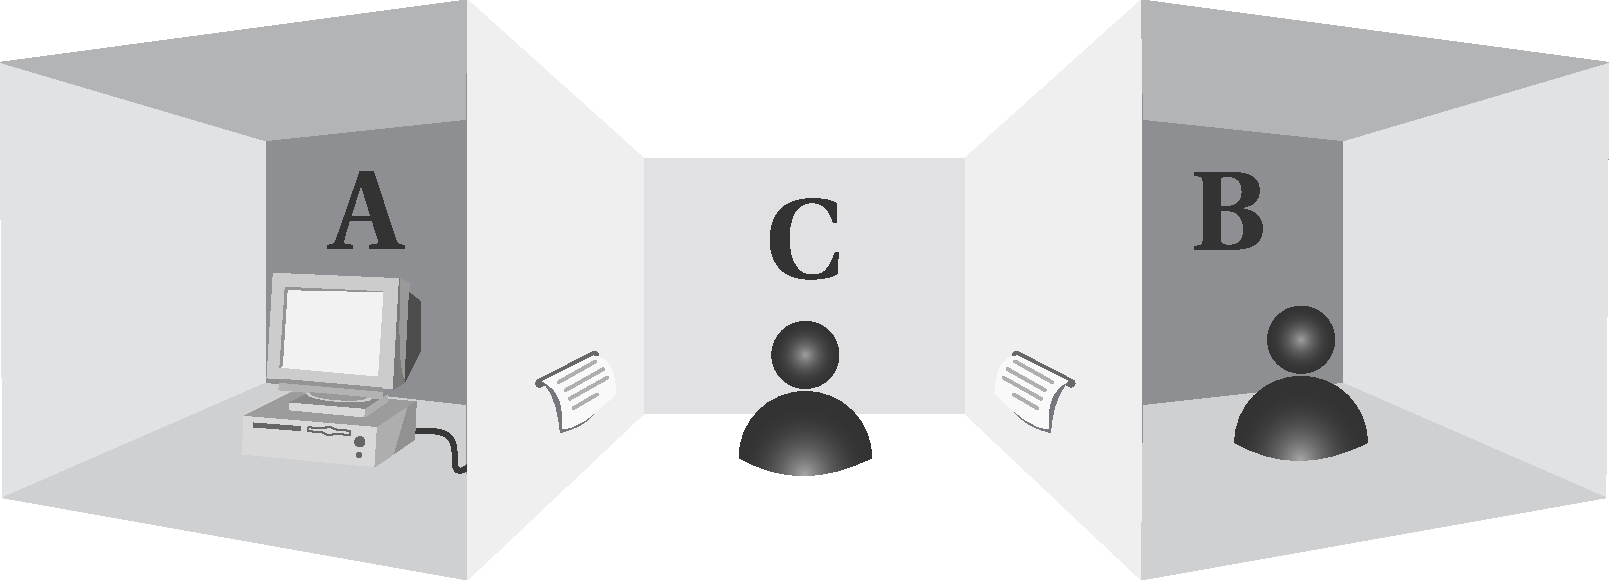
\includegraphics[width=0.6\textwidth]{Figures/Introduction/imit_game.pdf}
\caption{Illustration of the imitation game. A computer (A) and a person (B) answer questions posed by a human interrogator (C). Participant A aims at providing human-like answers, attempting to trick C into thinking that the answers were provided by a person.}
\label{fig:imitation_game}
\end{center}
\end{figure}

% Role of questions
While specific practical and philosophical limitations in the imitation game have been identified~\cite{turing2009computing,french1990subcognition}, it underscores the importance of language understanding and generation in machines. Moreover, it highlights the key role of questions and answers in evaluating the true intelligence of a machine. Additionally, beyond merely determining a machine's intelligence, the use of questions and answers represents a means of communication for the execution of specific tasks. An intelligent machine, as defined by the Turing test, not only communicates like a human but also possesses the capability to perform tasks akin to human abilities, rendering it versatile across a broad spectrum of applications, some of them in the field of medicine.

In order to emulate human behavior, the machine is expected to learn. While Turing explored some intriguing ideas such as the use of rewards and punishment in the learning process, it was not until the advent of \gls{ml} that machines began to perform tasks with a degree of acquired knowledge (\ie, \textit{learning}). This initiation occurred with the work of Arthur Samuel in the 1950s, where he proposed a learning method for the game of Checkers based on the optimization of a game tree~\cite{samuel1959some}. A major breakthrough occurred with the perceptron~\cite{rosenblatt1958perceptron}, a single-layer neural network with a linear threshold function, considered to be an essential building block of modern~\glspl{ann}. The perceptron updated its parameters using the difference between the output of the target. Stacking multiple perceptrons required the propagation of errors through the network, which was enabled with backpropagation~\cite{linnainmaa1970representation}. This advancement facilitated the training of multilayer perceptrons~\cite{werbos2005applications,rumelhart1986learning} and became the standard algorithm for error propagation. Together with gradient descent, it allows models to learn from experience. This stands in contrast to the traditional approach of programming models with pre-defined instructions for every conceivable input and state. 





% Introduce machine learning, link it to how Turing delineated the learning process of the machine as a kid
Returning to Turing's work, the aforementioned developments paved the way for machines to resemble the way in which humans learn from experience more closely. The process of learning to perform specific tasks, such as playing Checkers or Chess~\cite{hsu1999ibm}, marked only the beginning of Turing's notions into the realm of machine intelligence. As he articulated in his paper,

% Finish with quote?
\begin{quote}
    \textit{It can also be maintained that it is best to provide the machine with the best sense organs that money can buy, and then teach it to understand and speak English.}
\end{quote}

We now delve into the role of vision and language understanding in enabling the interrogation of a machine.

\subsection{Computer Vision and Language Processing}

\subsubsection{Perceiving the World}
% Switch to CV
% Applications to medicine
Providing machines with vision capabilities marked a significant stride toward realizing the machine intelligence envisioned by Turing. However, it is crucial to distinguish between image processing and computer vision. Image processing aims to enhance visual appearance, extract information, or transform images. On the other hand, computer vision is focused on recovering the \glsxtrshort{3d} structure of the world from input images and utilizing this information for full scene understanding~\cite{szeliski2022computer}. In essence, computer vision is concerned with understanding the reality expressed by an image or video. 

Early computer vision approaches were introduced in the 1970s with the goal of achieving comprehensive scene understanding. These approaches encompassed a diverse range of techniques, including \glsxtrshort{3d} structure inference from \glsxtrshort{2d} lines, line labeling, generalized cylinders, pictorial structures, and optical flow algorithms~\cite{szeliski2022computer}. In 1980, a network architecture named \textit{Neocognitron} emerged and was applied to handwritten character recognition, building upon earlier ideas derived from the visual nervous system. The concept involved cascading a series of alternating simple and complex cells, where the former was responsible for local feature detection, and the latter captured global patterns~\cite{fukushima1980neocognitron}. This pioneering work laid the groundwork for \glspl{cnn}~\cite{lecun1998gradient}, which share structural similarities with Neocognitron but are more flexible due to the use of generic convolution and pooling operations, facilitating the automatic extraction of hierarchical feature representations. Despite being formalized at the end of the twentieth century, the widespread application of these networks was hindered by hardware limitations~\cite{krizhevsky2012imagenet}. 

Starting around 2012, as a result of the developments in graphics processing units and parallelization, the utilization of \glspl{cnn} experienced exponential growth, witnessing the proposal of various architectures tailored for tasks like image classification, image segmentation, facial recognition, and image generation~\cite{bhandare2016applications}. More recently, an alternative architecture has emerged as a formidable contender to \glspl{cnn}. The \gls{vit}~\cite{dosovitskiy2020image} adapts an architecture originally designed for text processing to operate effectively with images. Both \glspl{cnn} and \glspl{vit} can be regarded as the closest approximation to the ``sense organs" envisioned by Turing. Attaining meaningful representations or descriptors of images represents a crucial step toward machines capable of performing tasks akin to human abilities. These architectures have also made substantial inroads into the medical domain, where they can, for example, contribute to alleviating the workload of clinical experts who may struggle to analyze all available images or benefit from a second opinion provided by a precise automated system.

However, models focused solely on vision are generally trained for specific tasks and often offer limited interaction, if any, with users. As Turing highlighted, imparting machines with the capability to understand and communicate in natural language is a crucial step forward.
% Now link this to Turing and state usefulnes for medical images

\subsubsection{Reading and Saying Words}

% start from computational linguistics
The desire for machines capable of understanding language is not a recent aspiration for humanity. In the mid-1930s, patents were conceived, with specific instances of translation machines~\cite{johri2021natural}. While rudimentary and basic, these can be considered the earliest practical ideas attempting language processing for a specific task. During the 1940s and 1950s, the challenge of machine language translation spurred initial research efforts, primarily following a rule-based design. Given the limited access to computers during this era, primarily research and military institutions could engage in such endeavors. Consequently and due to political interests, the main objective was to create machines capable of translating Russian text into English~\cite{hutchins1999retrospect}. Linguistic experts like Noam Chomsky identified limitations in translation systems during the 1950s, highlighting a lack of genuine comprehension of text content~\cite{chomsky1896chomsky}.% For example, sentences such as "Colorless green ideas sleep furiously" and "Furiously sleep ideas green colorless" were being categorized with the same degree of improbability, despite one of them being grammatically valid.

% The Eliza Program (1966)
Gradually, the applications of language transitioned from translation to dialogue, bringing the process a step closer to the imitation game, albeit with limited results. An illustration of this shift is ELIZA~\cite{weizenbaum1966eliza}, which engaged in simulated conversations with humans by utilizing reassembly and decomposition rules. This program, however, lacked a genuine understanding of the meaning of words.

% LUNAR (1972), SHRDLU
Years later, in 1970, as a response to the disappointment stemming from earlier works and with an aim to incorporate the meaning of words along with syntactical analysis and identification of lexical items, a program named SHRDLU was introduced~\cite{winograd1980does}. This program demonstrated the capability to answer basic questions, execute commands, and augment its knowledge about a simulated robot arm with access to toy objects. Subsequent systems further expanded the ability to answer questions to specific fields, such as lunar geology~\cite{woods1973progress}.

An important advancement in the representation of sequential information came about with \glspl{rnn}~\cite{rumelhart1986learning}. When coupled with the error propagation and parameter adjustment techniques mentioned earlier, \glspl{rnn} played a crucial role in enhancing the extraction of meaningful information from sequences and the sequential generation of data. The concept of mapping words to distributed vectorial representations that consider similarity~\cite{bengio2000neural} (\ie, word embeddings) marked a significant step, enabling the application of \glspl{rnn}, in all of its variations, to text sequences for various tasks.

More recently, the transformer architecture~\cite{vaswani2017attention} has revolutionized language processing by addressing limitations of \glspl{rnn} such as long-term dependencies, scalability and efficiency. This architecture, combined with substantial computing power and large text datasets, has paved the way for the conception and implementation of \glspl{llm}. \glspl{llm} are language models with a large number of parameters and trained on internet-scale datasets. In recent years, these models have evolved to the point of becoming prominent as information sources, chatbots, or assistants~\cite{pal2023chatgpt}. 

Having models that perceive the world and ``speak" a language seems to align with Turing's aspirations for the imitation game. However, devising a model that seamlessly integrates vision and language is not a trivial task, as it demands a certain level of correspondence between text and vision representations.

%*************************
% FROM HERE TO BE CORRECTED
%*************************

\subsection{Visual Questioning}
% Move to VL focusing on VQA
Endowed with vision and language capabilities, machines can perform a diverse array of tasks, such as image captioning, image retrieval, text-to-image generation, visual grounding, visual storytelling and \gls{vqa}. Notably, \gls{vqa} holds considerable appeal as it enables interaction between humans and machines through questions related to images or videos. Involving skills like spatial reasoning, logical inference, comparisons, counting, memorization, object and attribute recognition and transitive relation tracking, \gls{vqa} requires visual understanding at various levels~\cite{hudson2019gqa}. This enhanced visual understanding adds a dimension to the Turing test, allowing the assessment of a model's ability to comprehend and interpret visual information. In this scenario, the setup for the Turing test is expanded: Interrogator C poses questions about visual content, which participants A and B can perceive, and they provide answers. Similar to the standard Turing test, if the interrogator cannot reliably distinguish between human and computer responses, the machine is deemed to pass the test.   

% First, mention [35] and [18] from https://dl.acm.org/doi/abs/10.1145/1459359.1459412 (2009)
Early applications towards visual question systems can be traced back to 2003, where applications included real-time motion tracking for browsing surveillance videos~\cite{katz2003answering} and questions about news videos based on analysis of transcripts but informed by computer vision techniques~\cite{yang2003videoqa}. These systems, however, had inherent limitations, such as a restricted set of possible questions and the reliance on an external module for vision processing, neglecting the necessity for a joint understanding of both modalities.

% Mention https://dl.acm.org/doi/abs/10.1145/1459359.1459412 (2009) in detail
A few years later, the concept of \textit{Photo-based Question Answering} emerged as a more comprehensive task involving questions about objects within in an image~\cite{yeh2008photo}. As depicted in \fig~\ref{fig:photo_qa}, the system comprises three layers: the first layer matches the input image to web images and extracts structured data from multimedia databases, the second layer searches for appropriate answers in an internal repository, and the third layer delegates more complex questions to humans.

\begin{figure}[!ht]
\begin{center}
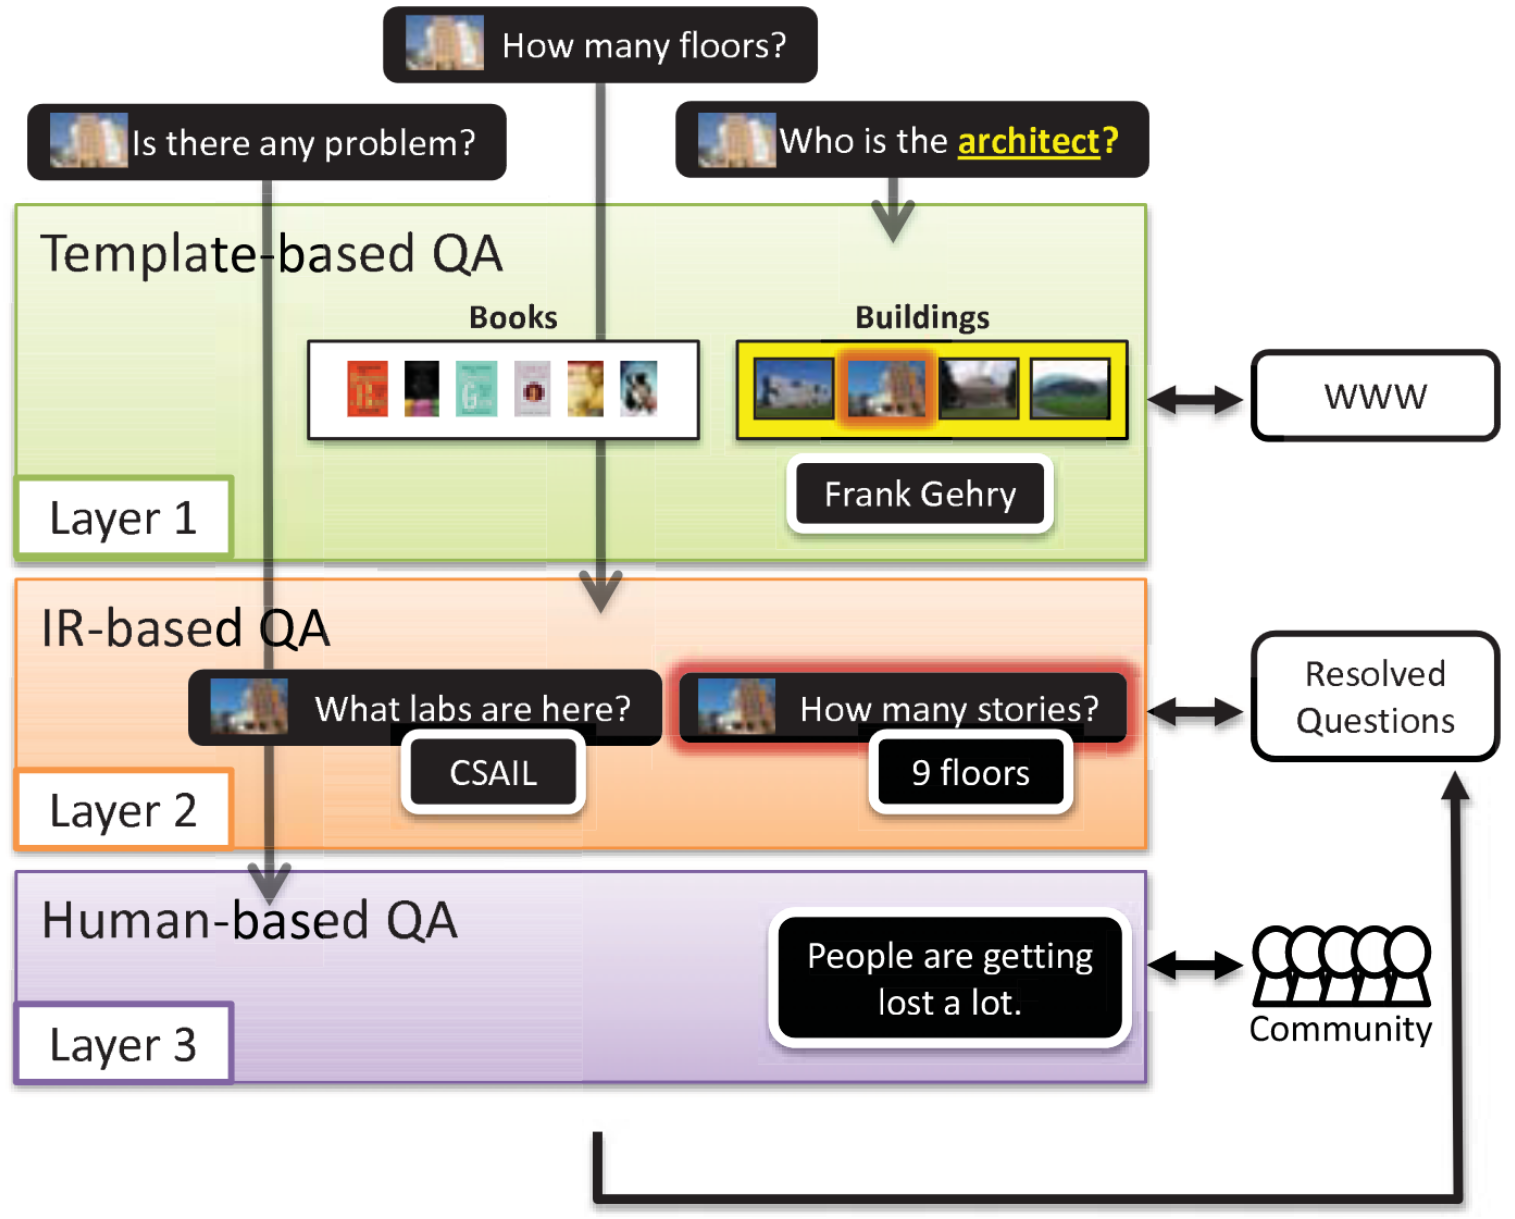
\includegraphics[width=0.5\textwidth]{Figures/Introduction/photo_qa.png}
\caption{A three-layer method for photo-QA. The first layer performs image matching of the input image to web images and extracts structured data. The second layer searches for applicable answers. The third layer allows humans to answer more complicated questions. From \cite{yeh2008photo}.}
\label{fig:photo_qa}
\end{center}
\end{figure}

% Mention papers that came before Antol et. al 2015!
% Jump to VizWiz 2010
A real-world application of visual questions emerged in 2010 with VizWiz~\cite{bigham2010vizwiz}, designed to provide visually impaired individuals with answers to questions about their daily interactions with the environment. Initially relying on crowd-sourced workers, the platform evolved to incorporate \gls{ai} solutions in subsequent years~\cite{gurari2018vizwiz,gurari2019vizwiz}. Notably, this application underscores the importance of free-form questions, allowing users to employ any grammatical structure to inquire about the contents of an image.

% Multi-world approach to... (2014) [30]
% Joint video and text parsing (2014) [42]
% VTT (2015) [16]
Further developments broadened the landscape in terms of datasets and methodologies. One approach enhanced the surveillance video browsing application mentioned earlier by utilizing a probabilistic model to capture relations between video and text using parse graphs~\cite{tu2014joint}. 

Another approach employed segmentation to gather facts about objects for answering template-generated questions from a limited vocabulary~\cite{malinowski2014multi}. Yet another formalized the concept of \gls{vtt} to evaluate the visual understanding of machines through a sequence of binary questions, ensuring that the history of questions and correct answers was unhelpful in answering the current question~\cite{geman2015visual}.

% Introduce VQA
The formal pursuit of answering visual questions gained momentum in 2015 with the introduction of the \gls{vqa} task. This challenge featured a dataset with thousands of open-ended human-generated questions about images~\cite{antol2015vqa} and presented an architecture as a baseline for benchmarking. The architecture comprised a frozen \gls{cnn} for image encoding, an \gls{rnn} for question encoding, a multiplication operation to combine both embeddings and an output classifier to select the most likely answer from a predefined list. Over time, the type of answer generated by models has evolved, with \glspl{llm} enabling the generation of more detailed answers and descriptions, aligning with Turing's vision of machines generating human-like responses.

Following the introduction of \gls{vqa} for natural images, the task found its way into the medical domain, garnering attention and inspiring researchers. Advancements in \gls{medvqa} have closely mirrored those in classical \gls{vqa}, with some exceptions for addressing data-related challenges and specialized architectures. A more detailed history of \gls{vqa} architectures and datasets is offered in Sec.~\ref{subsec:vqa_history}.

% To go into medicine, I could switch the question of the turing test to machine vs. doctor
Expanding on this trajectory, we can envision a variation of the Turing test for medical images. In this scenario, participants B and C are replaced by experts in a specific medical imaging modality, with A being the machine. Interrogator C poses medical questions about images to A and B. If C tends to believe that A is a medical expert with high probability, the machine could be deemed intelligent in a medical sense, showcasing specialized knowledge beyond general human knowledge. In this context, the accuracy of answers and the terminology used play a crucial role, demanding more from the machine to simulate a medical expert compared to simulating a human. One case in which this simulation can fail is when the machine provides contradictory answers too often. Following this line of thought, we briefly examine the case in which two questions are asked about the same image.

% End with questions about whether or not models are actually reasoning or what level of reasoning they have

\section{Making Sense}

% Can machines think? Go back to Turing paper
% Possible example. Ask two questions about basic knowledge
% e.g.  Abraham Lincoln lived between 1809 an 1865 ->  he lived in the 19th century
% A model that says he lived in those years and also says he's from the 18th century is being inconsistent
Given that humans are prone to errors, it is reasonable to expect a machine emulating human behavior to also make mistakes, especially when faced with challenging tasks that allow only limited generalization to unseen examples post-training, introducing errors in responses. However, in the imitation game, the nature of errors made by A and B can significantly impact C's final identification of the participants as machine or human. 

Illustrating this with the text-only Turing test, consider the following example. If we query the machine about the years Abraham Lincoln was alive and receive the correct response "1809 to 1865," but then ask about the century and get the incorrect answer "18th century," we identify an issue beyond mere errors. Abraham Lincoln being alive both in 1809 - 1865 and in the 18th century is a contradiction. Asking about the same information, we expect a machine (as we do a human) to avoid contradictions in responses, displaying \textit{consistency}.

Detecting such contradictions, a skill innate to humans, proves challenging for machines but directly influences the quality of reasoning they employ~\cite{selvaraju2020squinting}. Reasoning, involving ``scaling to ever-larger search spaces and understand the world broadly," implies consistency, causality, and compositionality~\cite{kervadec2021bias}. The absence of any of these elements can cast doubt on the quality of reasoning.

% key point: Evaluating propositions to true or false often requires external information. In the case of the images, this can be achieved more easily than for text. That's why it's easier to evaluate logical reasoning when images are available
Incorporating images into the imitation game facilitates testing the model's consistency, as queries can reference external visual evidence. In the text-only scenario, a comprehensive image description (objects, relations, color, structure, \etc) would be needed in the question, creating a challenge. For instance, consider presenting a \gls{vqa} model with an image of a bear statue and asking: "What is this?" and "Is it alive?" If the model responds "a statue of a bear" and "yes," respectively, inconsistent behavior becomes apparent. Humans leverage logic and prior knowledge, understanding that a statue cannot be alive. Thus, ensuring machine consistency requires integrating logical faculties, explicitly or implicitly.


In the medical domain, the significance of consistent answers amplifies due to the potential impact on medical decisions. The adoption of \gls{medvqa} systems by medical experts hinges on trust, with models demonstrating less contradictory behavior being perceived as more trustworthy and effective tools.


\section{Thesis Statement}

This thesis addresses visual understanding and reasoning in \gls{vqa} by means of two perspectives:

\begin{enumerate}
    \item Localized queries, where questions can be posed about any region of an image,
    \item Consistency enhancement, where a model is encouraged to avoid contradictions,
\end{enumerate}

respectively. Considering this, we formulate the following thesis statement:

\textit{\textbf{Achieving high-quality clinical decisions through Visual Question Answering systems requires a prioritization of consistency and fine-grained queries, offering a pathway to improved spatial understanding and overall model reliability.}}

% Tatiana
%Machine learning techniques can be successfully used to make clinical practice safer, but validation that goes beyond conventional performance metrics is crucial to provide the in- sight needed in order to assess a method’s reliability.
%Tom
%AI-based medical assistants can perform tasks as well as medical experts, can perform tasks magnitudes faster and can perform tasks impossible for humans.
% Laurent
%Generating pixel-wise annotations of medical sequences over a wide range of modalities is greatly facilitated by means of a novel fast and intuitive protocol that relies on sparse point-wise cues, aided by a segmentation framework that relies on DL and multi-object tracking.

% Possible thesis statements

% - Achieving high-quality clinical decisions through Visual Question Answering systems requires a prioritization of consistency and localized queries, offering a pathway to improved spatial understanding and overall model reliability.

% - Consistency and localized questions play a fundamental role in the trustworthiness and performance evaluation of VQA models, offering valuable insights into the reasoning capabilities and visual understanding

% - Visual Question Answering systems can contribute to the quality of clinical decisions, but they require consistency and local queries to unlock better consistency and spatial understanding. 

% - Unlocking the potential of Visual Question Answering models for clinical decision-making hinges on prioritizing consistency and incorporating localized queries, ushering in advancements in spatial understanding and the overall reliability of the system.

\section{Organization and Contributions of the Thesis}


Chapter~\ref{chapter:background} lays the foundation with key concepts related to language and vision, along with their combination. The chapter delves into \gls{nlp}, highlighting its prominent architectures, and focuses on pivotal aspects of computer vision, emphasizing \glspl{cnn} and \glspl{vit}. \glspl{vlm} are then explored, followed by an in-depth examination of \gls{vqa} from both architectural and data perspectives. Additionally, basic concepts regarding \gls{dme} staging are presented, due to their relevance in this thesis.

Part~\ref{part:localized} is dedicated to the exploration of localized questions (\ie, questions about specific image regions) in \gls{vqa}. Chapter~\ref{chapter:locvqa} introduces a method enabling such questions for \gls{vqa} models with guided attention mechanisms. The proposed approach involves localized attention, integrating a target region represented by a binary mask into the \gls{vqa}'s attention mechanism. This enables the model to compute attention maps on the entire image, subsequently filtering them spatially to focus on the specified region. Experiments on multiple datasets demonstrate the method's potential applicability.

Chapter~\ref{chapter:locvqallm} extends the concept of localized questions to \glspl{mllm}. The proposed targeted visual prompting involves creating a customized visual prompt containing the isolated region and the region in context. Visual components of the prompt are processed by a Swin Transformer and then projected into the input space of the \gls{llm}. Comprehensive experiments highlight the method's benefits across various medical \gls{vqa} datasets. 

Part~\ref{part:consistency} introduces two works in the field of consistency for \gls{vqa}. The approach in Chapter~\ref{chapter:cons_mainsub} exploits the categorization of questions into perception and reasoning based on the visual abilities demanded from the model to answer them. This categorization informs a loss function term, enforcing consistency by penalizing inconsistent cases during training. The result is an improvement in both consistency and accuracy, showcasing the advantages of such model-agnostic approaches. 

Chapter~\ref{chapter:cons_logic} builds upon the previous work by revising the definition of consistency and formalizing it from a more general perspective using logical implications. Similar to the prior method, a loss term is used to optimize consistency during training, encouraging the model to correct inconsistencies without compromising overall performance. Since implication annotations are usually not included in \gls{vqa} datasets, we propose to predict them by leveraging a language model trained for the task of \gls{nli}. Evaluation on medical and non-medical datasets supports the effectiveness of the approach compared to state-of-the-art consistency enhancement methods.

Finally, Part~\ref{part:discussion_future} contains a discussion and summary of the findings and limitations of the works presented in the thesis (Chapter~\ref{chapter:discussion_conclusion}), and offers possible directions for future work (Chapter~\ref{chapter:future_work}).

%\begin{figure}[!ht]
%\begin{center}
%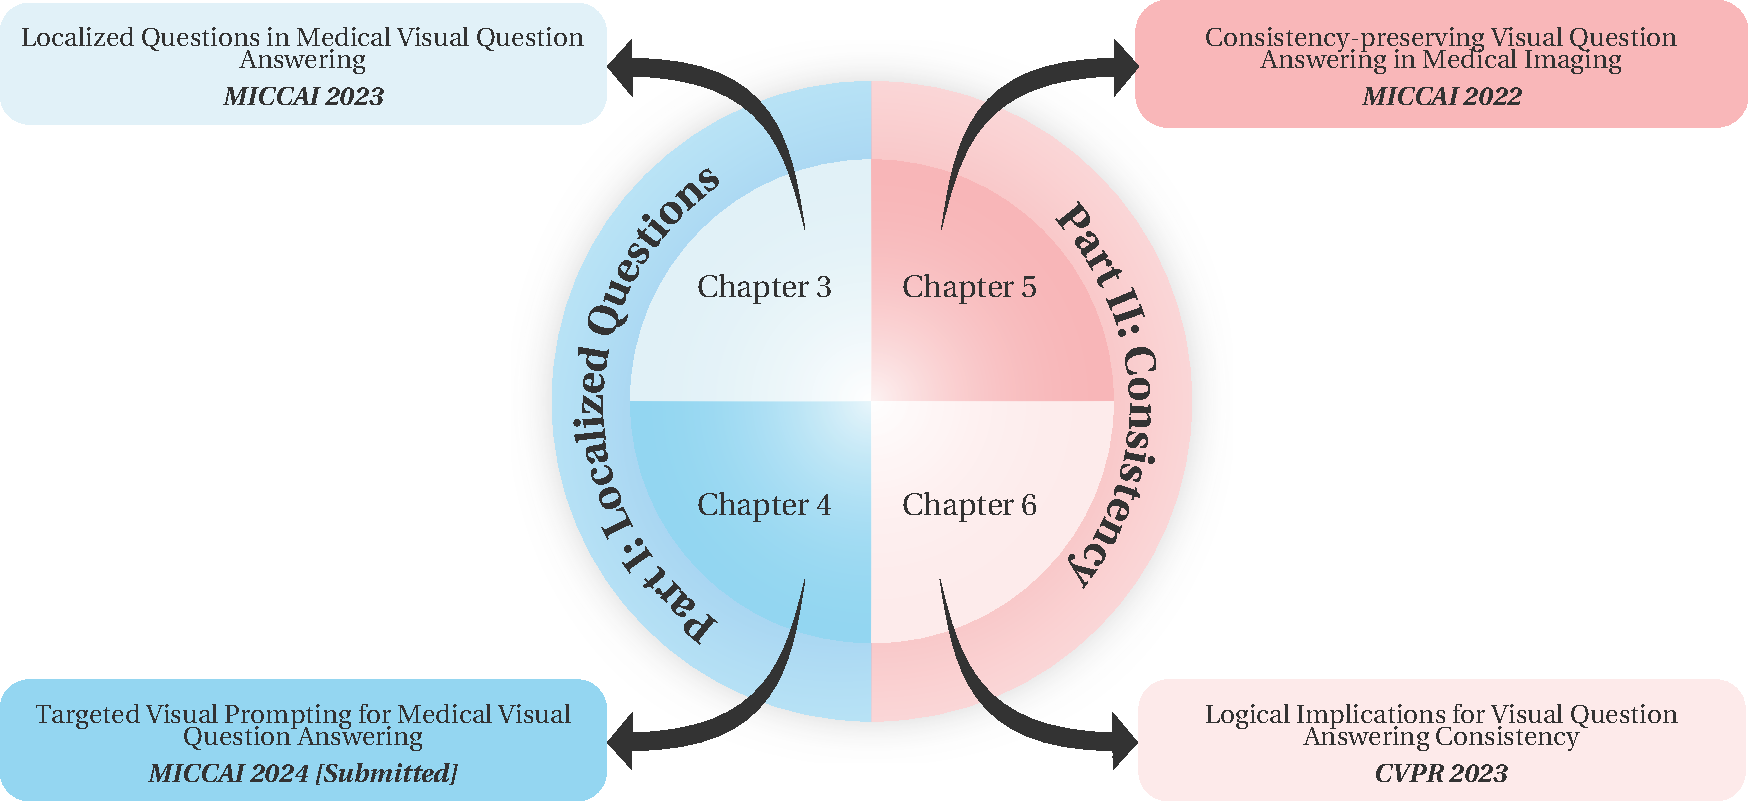
\includegraphics[width=\textwidth]{Figures/Introduction/manuscript_organization.pdf}
%\caption{Organization of the contributions of the manuscript.}
%\label{fig:manuscript_organization}
%\end{center}
%\end{figure}

